\chapter{Modes propres}
On peut maintenant implémenter le problème aux valeurs propres du chapitre \ref{eigen} afin de trouver les couples $(\lambda_i,\bm{g_i})$ tel que $\rot\bm{g_i}=\lambda_i\bm{g_i}$ pour $i=1,\dots,M$. Les fonctions propres seront la base sur laquelle on va projeter $\bm{u}$ pour la décomposition de Galerkin \[ \bm{u}=\sum_{i=1}^M c_i\bm{g_i} \]
Comme les fonctions propres vivent dans $D^1$, un espace à divergence nulle, l'opérateur rotationnel et le laplacien sont identiques. Cependant, comme les fonctions tests implémentées dans Feel++ ne sont pas à divergence nulle, si on utilise le laplacien, il est nécessaire de rajouter une étape de tri pour avoir des fonctions à divergence nulle. Comme cela est très coûteux en temps de calcul, il vaut mieux utiliser directement l'opérateur rotationnel.

\section{Cas général}
Ici, on veut s'appuyer sur les travaux de V. Girault \cite{girault90-1}. Pour cela, on a besoin de définir l'espace \[X = \{\bm{v}\in H(rot)\ |\ (\rot\bm{v}\cdot\bm{n})\restr=0 \}\]
On rappel les définitions suivantes :
\begin{align*}
L^2_\sigma(\Omega) &= \{\mathbf{v} \in L^2(\Omega)\ |\ \div \mathbf{v} = 0\text{ et }\mathbf{v}\cdot \mathbf{n}\restr = 0 \}\\
D^1(\Omega) &= \{\mathbf{v} \in H^1(\Omega)\cap L^2_\sigma(\Omega)\ |\ (\rot \mathbf{v}\cdot \mathbf{n})\restr = 0  \}
\end{align*}
De plus, on a (voir \cite{Girault79}) :
\[ H^1(\Omega)=H(rot)\cap H(div) \]
D'où:
\begin{align*}
D^1(\Omega) &= \{\bm{v}\in H^1(\Omega)\cap L^2_\sigma(\Omega)\ |\ (\rot \mathbf{v}\cdot \mathbf{n})\restr = 0  \}&\\
&=\{\bm{v}\in H(rot)\cap H(div)\cap L^2_\sigma(\Omega)\ |\ (\rot \mathbf{v}\cdot \mathbf{n})\restr = 0  \}&\\
&&\text{ or }L^2_\sigma\subset H(div)\\
&=\{\bm{v}\in H(rot)\cap L^2_\sigma(\Omega)\ |\ (\rot \mathbf{v}\cdot \mathbf{n})\restr = 0  \}&\\
&=\{\bm{v}\in H(rot)\ |\ (\rot \mathbf{v}\cdot \mathbf{n})\restr = 0  \}\cap L^2_\sigma(\Omega)&\\
&=X\cap L^2_\sigma(\Omega)&
\end{align*}

Le problème aux valeurs propres est :\\
Trouver $(\bm{g},\lambda)\in X\cap L^2_\sigma\times\R$ tel que :
\begin{align}
\rott\bm{g}&=\lambda^2\bm{g} \label{impPb1}\\
\div\bm{g}&=0 \label{impPb2}\\
(\bm{g}\cdot\bm{n})\restr&=0 \label{impPb3}\\
(\rot\bm{g}\cdot\bm{n})\restr&=0 \label{impPb4}\\
(\rott\bm{g}\cdot\bm{n})\restr&=0 \label{impPb5}
\end{align}
Mais les conditions (\ref{impPb2}-\ref{impPb3}) sont satisfaites par le fait que $\bm{g}\in L^2_\sigma$ et la condition (\ref{impPb4}) par l'appartenance à $X$.\\

En passant à la forme variationnelle, et en suivant les mêmes étapes que dans le chapitre (\ref{eigen}), on impose la condition (\ref{impPb5}) :
\[ \int_\Omega (\rot\bm{g})\cdot(\rot\bm{\varphi}) + \int_{\partial\Omega} \phi(\underbrace{(\rott \bm{g})\cdot\bm{n}}_{=0})= \lambda^2\int_\Omega \bm{g}\cdot\bm{\varphi} \]
On a donc le problème suivant :\\
Trouver $(\bm{g},\lambda)\in X\cap L^2_\sigma\times\R$ tel que $\forall \bm{\varphi}\in X\cap L^2_\sigma$ :
\[ \int_\Omega (\rot\bm{g})\cdot(\rot\bm{\varphi}) = \lambda^2\int_\Omega \bm{g}\cdot\bm{\varphi} \]

Ne pouvant pas utiliser directement des fonctions de bases à divergence nulle pour les éléments finis, on impose cette condition par un terme de pression fictif. On a donc :\\
Trouver $((\bm{g},p),\lambda)\in X\cap L^2_\sigma \times H^1 \times \R$ tel que $\forall (\bm{\varphi},q)\in X\cap L^2_\sigma \times H^1$ :
\begin{align*}
\int_\Omega (\rot\bm{g})\cdot(\rot\bm{\varphi}) + \int_\Omega\bm{\varphi}\grad p &= \lambda^2\int_\Omega \bm{g}\cdot\bm{\varphi}\\
\int_\Omega (\div\bm{g}) q &= 0
\end{align*}
En intégrant par partie la seconde équation, on obtient
\[ \int_\Omega (\div\bm{g}) q = \int_\Omega \bm{g}\grad q - \int_{\partial\Omega} (\underbrace{\bm{g}\cdot \bm{n}}_{=0})q = 0 \]
On peut donc imposer les contraintes (\ref{impPb2}-\ref{impPb3}), liées à $L^2_\sigma$, dans la formulation faible suivante :\\
Trouver $((\bm{g},p),\lambda)\in X \times H^1 \times \R$ tel que $\forall (\bm{\varphi},q)\in X \times H^1$ :
\[ \int_\Omega (\rot\bm{g})\cdot(\rot\bm{\varphi}) + \int_\Omega\bm{\varphi}\grad p + \int_\Omega \bm{g}\grad q = \lambda^2\int_\Omega \bm{g}\cdot\bm{\varphi} \]

Pour imposer la condition (\ref{impPb4}), on utilise une méthode de pénalisation, le problème devient donc :
Trouver $((\bm{g},p),\lambda)\in H(rot) \times H^1 \times \R$ tel que $\forall (\bm{\varphi},q)\in H(rot) \times H^1$ :
\begin{equation}\label{impFvEigen}
\int_\Omega (\rot\bm{g})\cdot(\rot\bm{\varphi}) + \int_\Omega\bm{\varphi}\grad p + \int_\Omega \bm{g}\grad q + \gamma\int_{\partial\Omega}(\rot\bm{g_i}\cdot\bm{n})(\rot\bm{\varphi}\cdot\bm{n}) = \lambda^2\int_\Omega \bm{g}\cdot\bm{\varphi}
\end{equation}
avec $\gamma$ une très grande valeur.\\

Ainsi, la solution se trouvant dans $H(rot)$, la meilleure méthode serait d'utiliser des éléments conformes à cet espace, à savoir les éléments de Nedelec. Cela permettrait d'avoir $\rot\bm{g_i}\in L^2(\Omega)$. On gagnerait ainsi en régularité sur les fonctions propres.

\subsection{Implémentation}

Cependant, les éléments de Nedelec n'étant pas prêt dans Feel++, on se place dans un espace plus large, $H^1$, et on utilise des éléments de Lagrange. Cela implique que $\rot\bm{g}$ n'appartient pas forcément à $L^2$. Cette méthode est donc moins précise et elle introduit de nouvelles erreurs de calcul.\\

Ces erreurs mènent à une divergence non nulle, on utilise donc un terme de pénalisation en plus afin de forcer la divergence. On résout donc le système suivant :
\[ \int_\Omega (\rot\bm{g})\cdot(\rot\bm{\varphi}) + \int_\Omega\bm{\varphi}\grad p + \int_\Omega \bm{g}\grad q + \gamma\int_{\partial\Omega}(\rot\bm{g_i}\cdot\bm{n})(\rot\bm{\varphi}\cdot\bm{n}) + \alpha\int_\Omega \div\bm{g}\div\bm{\varphi} = \lambda^2\int_\Omega \bm{g}\cdot\bm{\varphi} \]

Cependant, on a toujours la condition $\bm{g}\cdot\bm{n}$ qui n'est pas respecter. On ajoute donc un troisième terme de pénalisation :
\begin{align*}
\int_\Omega (\rot\bm{g})\cdot(\rot\bm{\varphi}) &+ \int_\Omega\bm{\varphi}\grad p + \int_\Omega \bm{g}\grad q & \\
&+ \gamma\int_{\partial\Omega}(\rot\bm{g_i}\cdot\bm{n})(\rot\bm{\varphi}\cdot\bm{n}) & (\ref{impPb4})\\
& + \alpha\int_\Omega \div\bm{g}\div\bm{\varphi} & (\ref{impPb2})\\
&+ \beta\int_{\partial\Omega}\bm{g_i}\cdot\bm{n})(\bm{\varphi}\cdot\bm{n})  = \lambda^2\int_\Omega \bm{g}\cdot\bm{\varphi} & (\ref{impPb3})
\end{align*}

Comme on cherche les solutions dans $[H^1(\Omega)]^3$, on utilise des éléments de Lagrange et non de Nedelec pour approcher les $\bm{g_i}$. Pour le terme de pression fictif, on utilise aussi des éléments de Lagrange, scalaire et d'ordre 1.\\ 
\lstinputlisting[linerange=space]{../../src/eigenprob.hpp}
Pour résoudre le problème $Ax=\lambda Bx$, on initialise $B$ comme une matrice de masse. On utilise pour cela une forme bilinéaire :\\
\lstinputlisting[linerange=rhsB]{../../src/eigenprob.cpp}
On ajoute maintenant les termes 
\[ \int_\Omega \rot \bm{g}\cdot\rot\bm{\varphi} + \int_\Omega\bm{\varphi}\grad p + \int_\Omega \bm{g}\grad q \]
à une autre forme bilinéaire qui formera la matrice $A$ :
\lstinputlisting[linerange={acurl,presgrad}]{../../src/eigenprob.cpp}
Afin de pouvoir contrôler les paramètres de pénalisation, on les ajoute en tant qu'options :
\lstinputlisting[linerange=options]{../../src/eigenprob.cpp}
On peut maintenant rajouter les trois termes de pénalisations :
\lstinputlisting[linerange={divdiv,bccurln,bcn}]{../../src/eigenprob.cpp}
Les deux matrices étant prêtes, on peut maintenant appeler une routine SLEPc pour résoudre le problème aux valeurs propres.
\lstinputlisting[linerange=eigen]{../../src/eigenprob.cpp}
Le solveur et le pré-conditionneur sont définis en tant qu'options, on peut donc les changer à l'exécution. Par défaut, on utilise un solveur itératif de type Krylov-Schur (voir \ref{arnoldi}), avec une transformation de type \emph{shift and invert} qui facilite la recherche des valeurs propres de plus petites magnitudes, cependant cette transformation est directe et risque donc de poser des problèmes lorsqu'on cherchera un très grand nombre de valeurs propres.

\subsection{Résultats}
Une fois les termes de pénalisation appliqués avec $\alpha=\beta=\gamma=1000$, les conditions imposées sont respectés.
\begin{center}
\begin{tabular}{ >{$}c<{$} | >{$}c<{$} | >{$}c<{$} | >{$}c<{$} | >{$}c<{$} }
\no & \lambda^2 & \div\star & \star\cdot\bm{n} & \rot\star\cdot\bm{n} \\ \hline
0 & 40.9302 & 0.00210937 & 0.0232026 & 0.185115 \\ \hline
20 & 62.7893 & 0.00142931 & 0.00150083 & 0.0948699 \\ \hline
30 & 72.3563 & 0.00236504 & 0.0244683 & 0.240543 \\ \hline
45 & 90.406 & 0.00354548 & 0.0201967 & 0.32537
\end{tabular}
\end{center}

La figure \ref{resultats} montre ces modes.

\begin{figure}[H]
	\makebox[\textwidth][c]{
		\subfloat[mode 0]{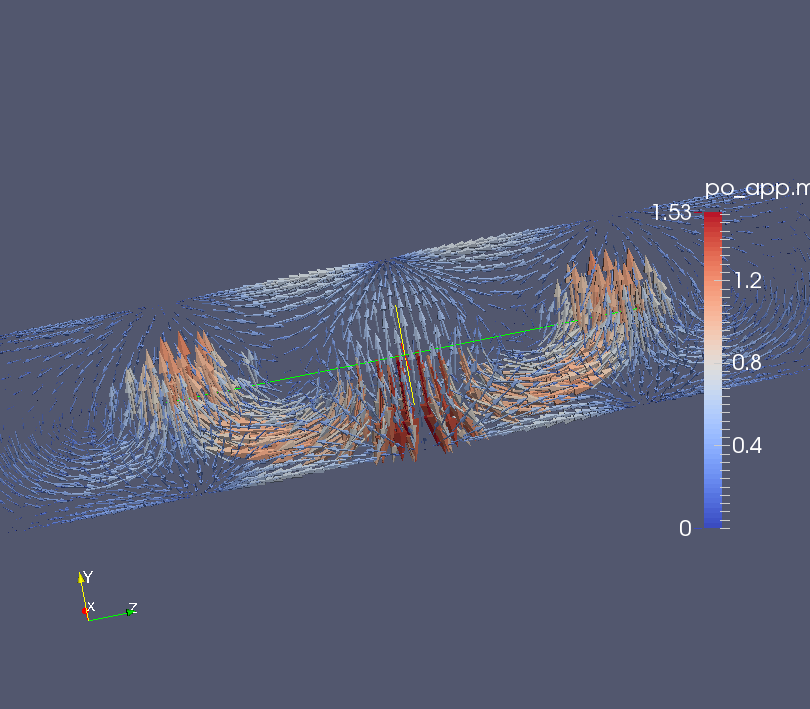
\includegraphics[scale=0.3]{curl-grad-1e3-mode0}}\ 
		\subfloat[mode 20]{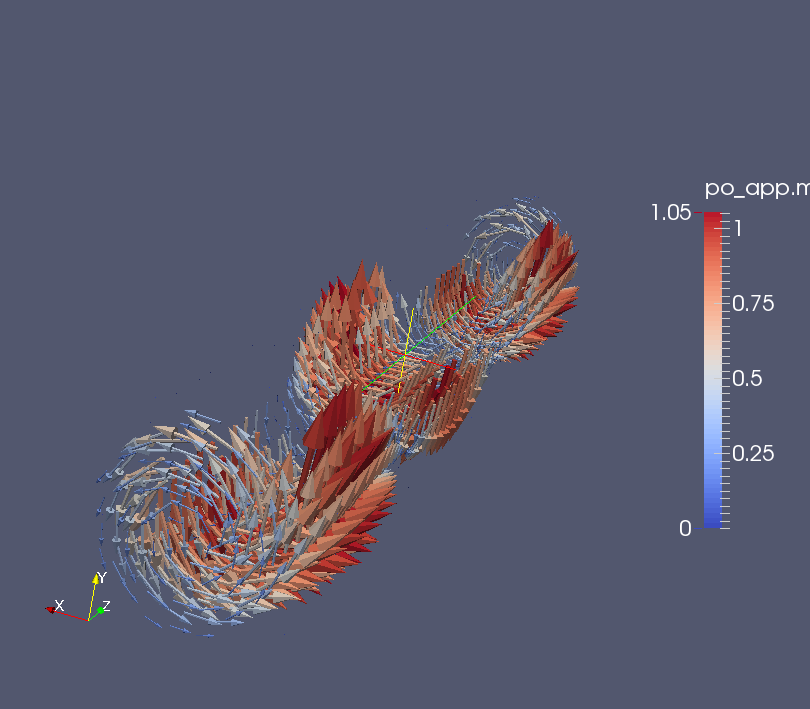
\includegraphics[scale=0.3]{curl-grad-1e3-mode20}}
	}\\
	\makebox[\textwidth][c]{
		\subfloat[mode 30]{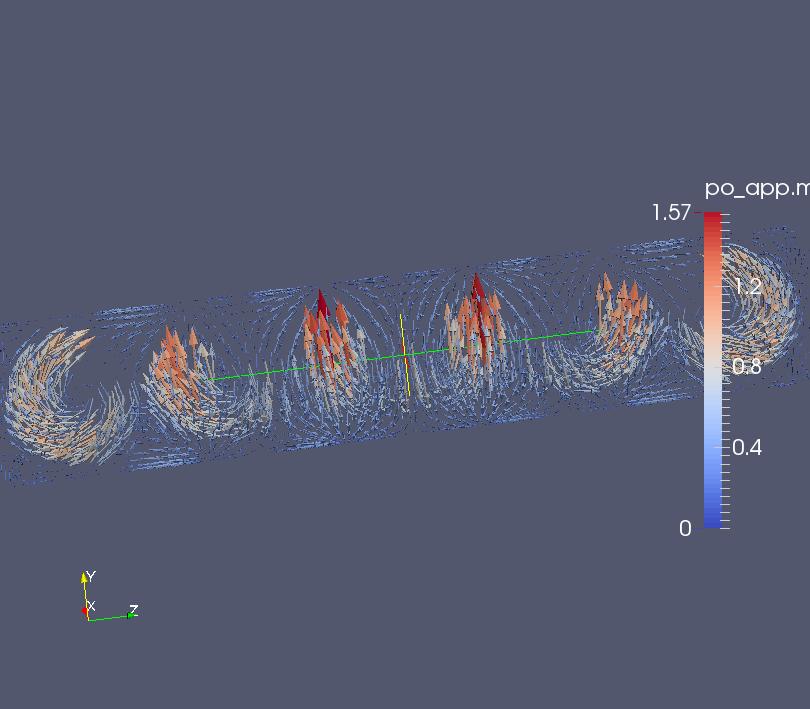
\includegraphics[scale=0.3]{curl-grad-1e3-mode30}}\ 
		\subfloat[mode 45]{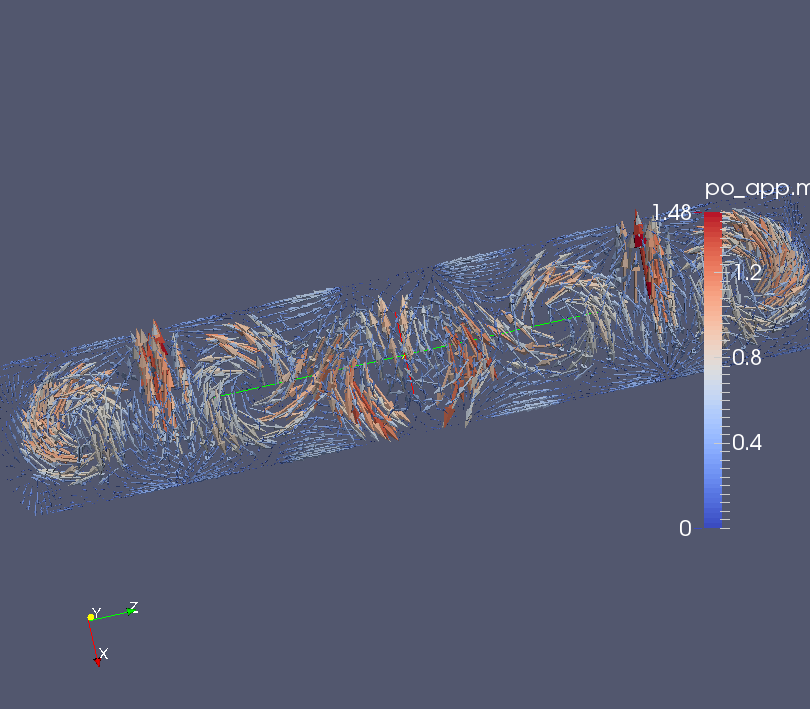
\includegraphics[scale=0.3]{curl-grad-1e3-mode45}}
	}
	\caption{Modes propres}
	\label{resultats}
\end{figure}
\todo[inline]{explication mode corrects}
Cependant, dû au manque de régularité de $\rot\bm{g_i}$, le calcul du rotationnel induit de grandes erreurs. Ainsi si on calcul l'erreur entre le rotationnel du champ et le champ multiplier par sa valeur propre, ou même lors du calcul de la condition $\rot\bm{g_i}\cdot\bm{n}$, on n'obtient pas les résultats escomptés :
\begin{center}
\begin{tabular}{ >{$}c<{$} | >{$}c<{$} | >{$}c<{$} | >{$}c<{$} | >{$}c<{$} | >{$}c<{$} | >{$}c<{$} | >{$}c<{$} | >{$}c<{$} }
\no & \lambda^2 & \lambda & \div\star & \star\cdot\bm{n} & \rot\star\cdot\bm{n} & ||\rot\star-\star|| & ||\star|| & ||\rot\star|| \\ \hline
10 & 49.1504 & 7.0107 & 0.00217561 & 0.0250946 & 0.208425 & 9.62716 & 0.999049 & 6.94417
\end{tabular}
\end{center}

De plus, en regardant les deux champs, on voit qu'ils n'ont pas la même forme. Par exemple, la figure \ref{eigendiff} montre la différence entre le 10\ieme\ vecteur propre et son rotationnel :

\begin{figure}[H]
	\makebox[\textwidth][c]{
		\subfloat[mode 10]{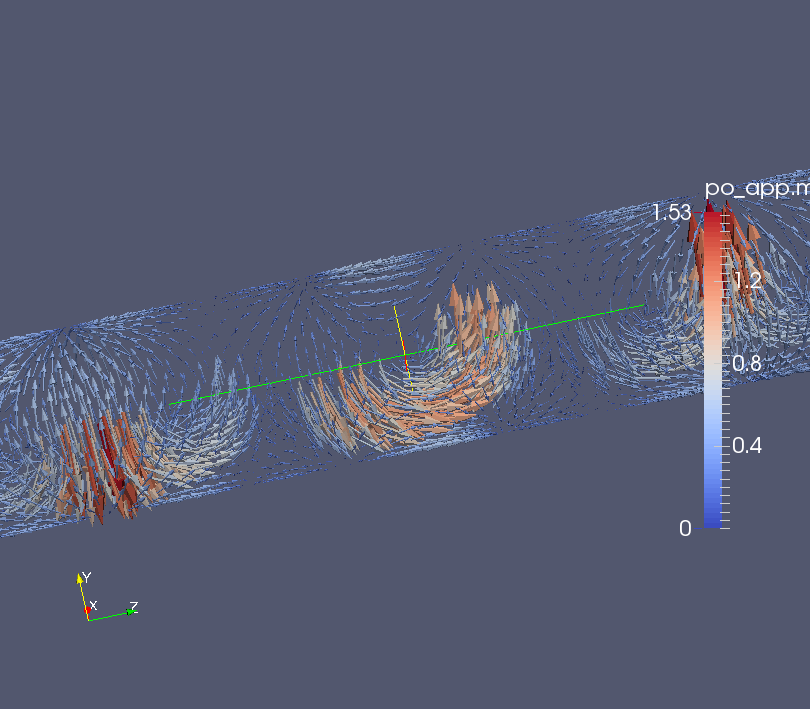
\includegraphics[scale=0.3]{mode10}}\ 
		\subfloat[$\rot($mode 10$)$]{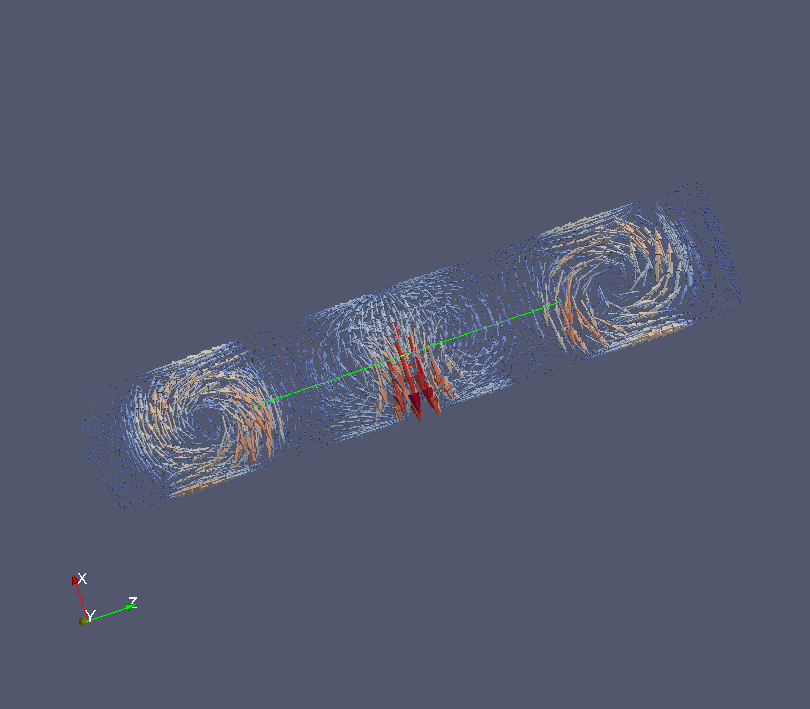
\includegraphics[scale=0.3]{curl10}}
	}
	\caption{Différences entre les modes et leur rotationnel}
	\label{eigendiff}
\end{figure}
Ces erreurs empêchent la vérification des résultats mais comme tous les calculs sur le rotationnel des modes propres sont remplacés par des calculs sur les fonctions propres multipliées par leur valeur propre respective, cela n'empêche pas la suite de la résolution du problème.\\

%% Cela peut aussi être dû aux paramètres de pénalisation, en effet si on change ces paramètres, on trouve des valeurs propres complètement différentes :

%% \begin{center}
%% \begin{tabular}{ >{$}c<{$} | >{$}c<{$} | >{$}c<{$} | >{$}c<{$} | >{$}c<{$} | >{$}c<{$} | >{$}c<{$} }
%% \alpha & \beta & \gamma & \lambda^2 & \div\star & \star\cdot\bm{n} & \rot\star\cdot\bm{n} \\ \hline
%% 0 & 0 & 0 & 5.24707e-11 & 15.0503 & 0.477078 & 1.23413e-07 \\ \hline
%% 10^3 & 10^3 & 10^3 & 40.9302 & 0.00210937 & 0.0232026 & 0.185115 \\ \hline
%% 10^6 & 10^6 & 10^6 & 57.1154 & 0.000159613 & 0.000673913 & 0.466915 \\ \hline
%% 10^{10} & 10^{10} & 10^{10} & 61.731 & 1.3273e-06 & 6.06696e-06 & 0.847356 \\ \hline
%% 10^{15} & 10^{15} & 10^{15} & 1.36827 & 2.30829e-09 & 5.37688e-08 & 5.57285 \\ \hline
%% 10^{10} & 10^3 & 10^3 & 42.0751 & 6.2461e-09 & 0.0310199 & 0.299304 \\ \hline
%% 10^3 & 10^{10} & 10^3 & 42.0096 & 0.00280563 & 0.0302683 & 0.280824 \\ \hline
%% 10^3 & 10^3 & 10^{10} & 57.5605 & 0.00622557 & 1.23812e-06 & 0.621214
%% \end{tabular}
%% \end{center}

%% Il y a donc un problème dans la méthode de pénalisation. Une explication pourrait être que les différents termes de pénalisation sont largement supérieurs aux termes correspondant au problème aux valeurs propres, et donc on ne résoudrait plus ce problème, mais un problème où la majorité des informations serait contenues dans les termes de pénalisation.\\

\subsection{Temps de calculs}
La figure \ref{tpsMode} montre les temps de calculs en fonction du nombre de modes propres, entre 1 et 100, pour différentes tailles de maillage.\\
Ces tests on été effectués sur une machine virtuelle Linux Debian 6, invitée sur un ordinateur avec 4 processeurs Intel Xeon cadencés à 2,4 GHz et 64 Go de RAM, mais avec seulement 47 Go de RAM alloués à la machine virtuelle.\\
J'ai effectué les tests sur les maillages suivants avec des éléments de Lagrange d'ordre 3 vectoriel pour $\bm{g}$ et d'ordre 1 scalaire pour $p$. \\

\begin{center}
\begin{tabular}{c|c|c|c}
taille du maillage & nombre d'éléments & Degré de liberté & Degré de liberté/proc\\ \hline
0,15 & 5000 & 80000 & 20000\\ \hline
0.125 & 7500 & 125000 & 30000\\ \hline
0.1 & 12500 & 200000 & 50000
\end{tabular}
\end{center}

\begin{figure}[H]
\centering
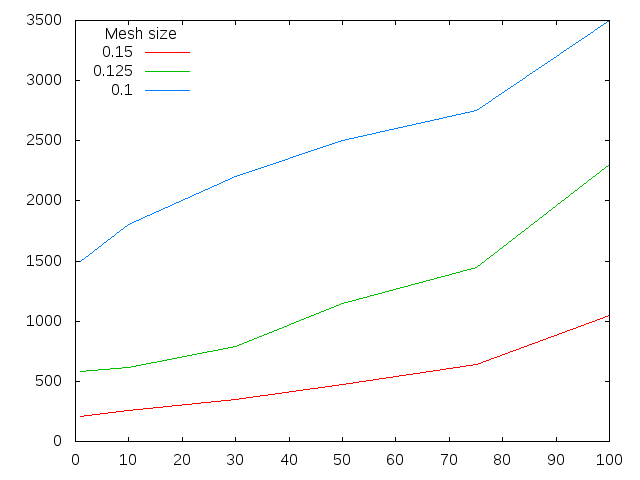
\includegraphics{tpsMode}
\caption{Temps de calcul en fonction du nombre de modes propres}
\label{tpsMode}
\end{figure}

% \section{Composante $z$}
% \subsection{Implémentation}
% \subsection{Résultats}

%%% Local Variables:
%%% TeX-master: "../report.tex"
%%% eval: (flyspell-mode 1)
%%% ispell-local-dictionary: "french"
%%% End:
